%*******10********20********30********40********50********60********70********80

\hypersetup{
    colorlinks=true,
    linkcolor=blue,
    filecolor=magenta,      
    urlcolor=blue,
}

% For all chapters, use the newdefined chap{} instead of chapter{}
% This will make the text at the top-left of the page be the same as the chapter

\chap{Development Method}
\section{Development Flow}

\textbf{1st Phase: Data collection and validation}\\
During this phase the most important thing is to gather as much as possible data, but they must be as much as possible reliable and useful since they are going to be indispensable for the next phases and in particular for the final results and conclusions.\\
The data’s reliability mainly depend by the kind of sources where you’re able to mine.\\
Then you should customize the unstructured data that you collected.\\
This data’s customizing has the main purposes of:
\vspace{-5mm}
\begin{itemize}
 \setlength{\itemsep}{-5pt}
 \item Let the data structure be a summarize of all the data inputs previous collected.
 \item Let the new data structure be easier to access and read.
 \item Follow some kind of setting and standard needed in the system that will be implemented.
\end{itemize}


\textbf{2nd Phase: Data Analysis and Displaying}\\
During this phase the first thing that you’re going to do is to decide some kind of analysis results that you would like to have.\\
Once you decided which kind of results you might reach, you will start with the analysis system implementation and meanwhile saving eviences of it.\\
Once the general analysis of the data is finished, and evidences have been collected, it's time to analyze it and try to extract information about it.

\newpage

\textbf{3rd Phase: Data Prediction}\\
During this phase the main purpose is to predict some kind of useful data about the current dataset. To reach this goal, is first of all indispensable to choose a prediction system to implement. \\
Once the prediction system has been implemented, it's time to apply it on the current data and try to get as much evidences as possible. \\

\textbf{4th Phase: Future Work ideas}\\
The last but not least phase is to watch at the future: try to figure out some other extra implementations about this thesis.\\


\begin{figure}[h]

    \makebox[\textwidth][c]{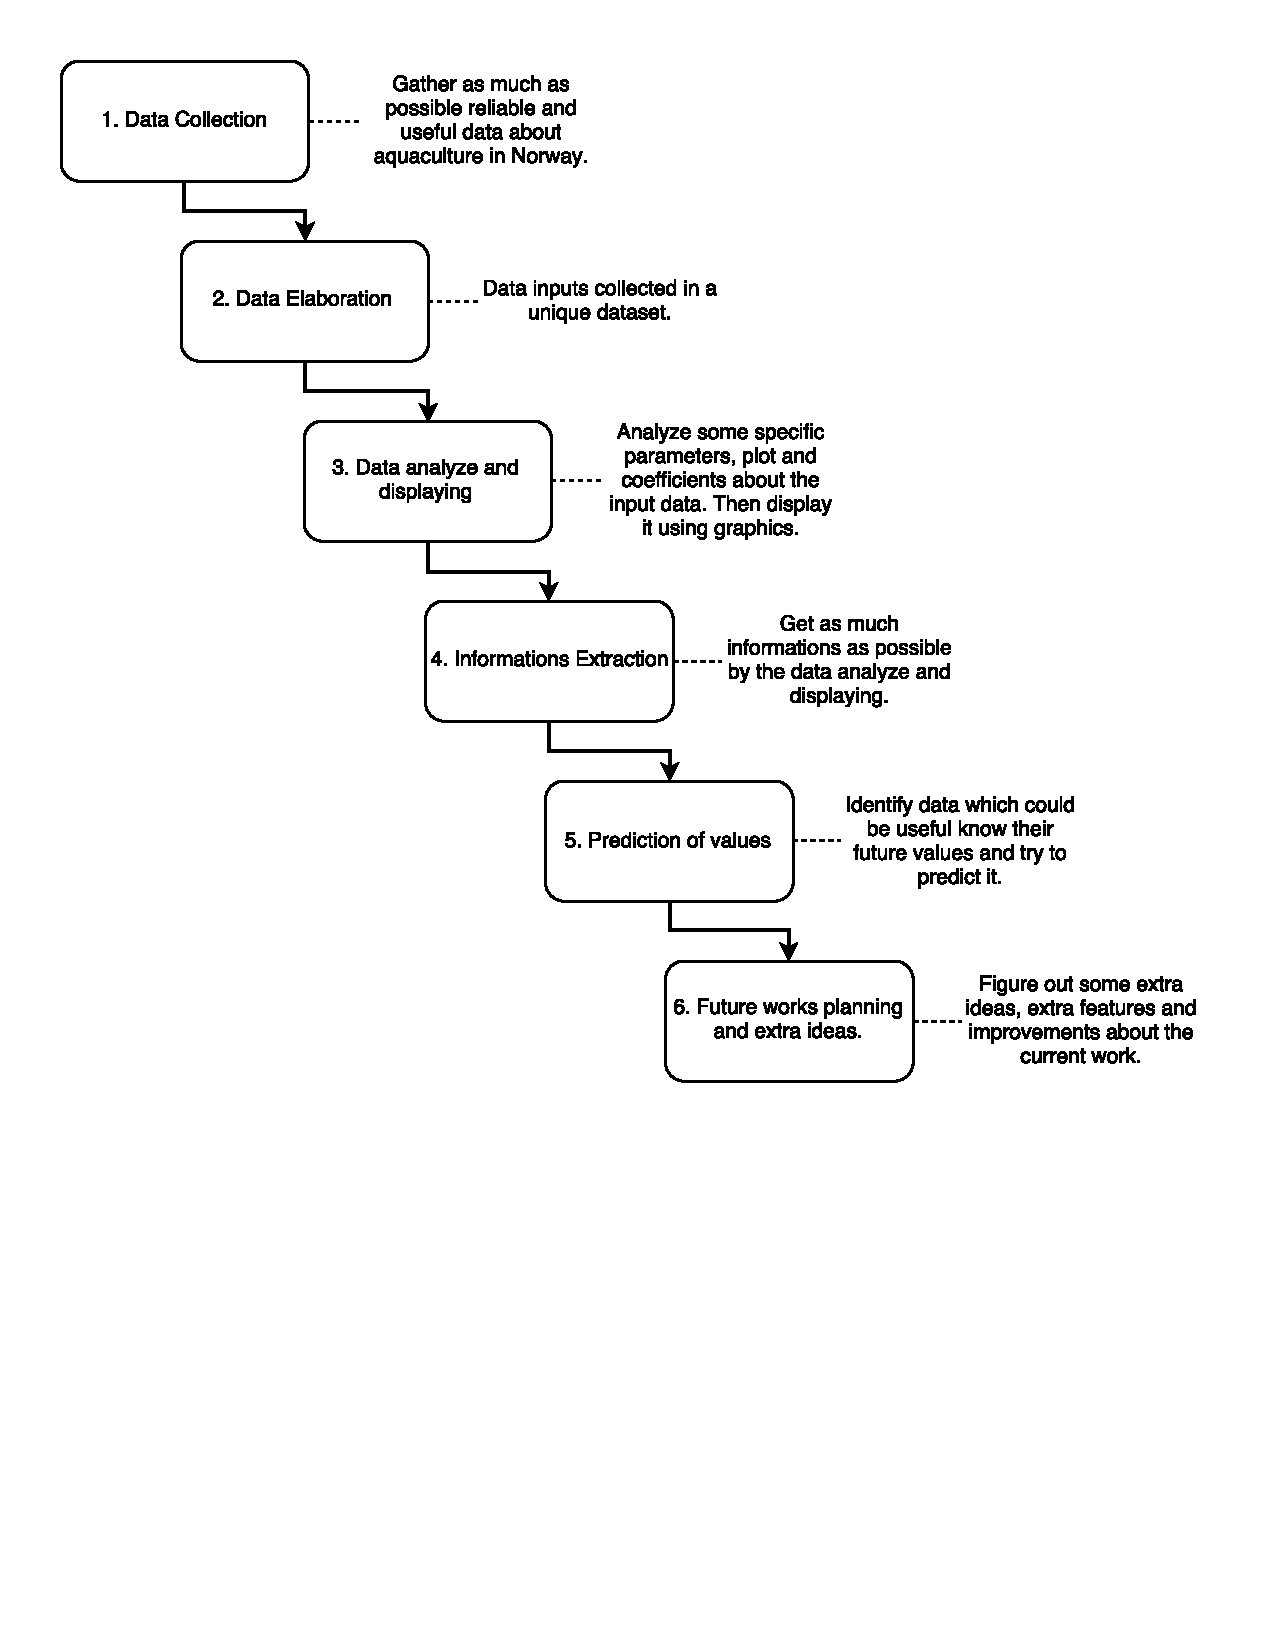
\includegraphics[width=1.2\textwidth,natwidth=761,natheight=681]{Files/DevelopmentFlow.pdf}}
    \caption[Plan flow chart]{Plan flow chart}
    \label{fig: Development_Flow}
\end{figure}

\newpage 
\section{Github Usage}
GitHub is a code hosting platform for version control and collaboration. It lets you and others work together on projects from anywhere.

In this thesis it will be used like "version control" since I'm the only person working on it, and I created on myself three repositories that will be very useful for better understand the work done with this thesis.

Repository that contains the Latex document about my thesis.\\
\url{https://github.com/Sprea22/Thesis_Latex_Doc}

Repository that contains the Data Analyzer implemented in python.\\
\url{https://github.com/Sprea22/Data_Analyzer_Python}

Repostory that contains the System for data forecasting implemented in python.\\
\url{https://github.com/Sprea22/Forecasting_System_Python}

Repostory that contains the System for map displaying.\\
\url{https://github.com/Sprea22/Norway_County_Analyzer}
